\documentclass[11pt]{article}
\usepackage[paperwidth=254mm,paperheight=142.875mm,margin=12mm]{geometry}
\usepackage{amsmath,amssymb}
\usepackage{graphicx}
\usepackage{booktabs}
\usepackage{xcolor}

\newcommand{\R}{\mathbb{R}}
\newcommand{\Var}{\operatorname{Var}}
\newcommand{\Cov}{\operatorname{Cov}}
\newcommand{\point}[2]{\item \textbf{#1}\par\vspace{3pt}{\centering #2\par}}
\newcommand{\plainpoint}[2]{\textbf{#1}\par\vspace{7pt}{\centering #2\par}\vspace{18pt}}
\newcommand{\hl}[1]{\colorbox{yellow!45}{$\displaystyle #1$}}

\newcommand{\slide}[1]{\clearpage\noindent{\Large\bfseries #1}\par\vspace{4pt}\hrule\vspace{10pt}}

\begin{document}

% TITLE SLIDE
\clearpage
\vspace*{\fill}
\begin{center}
{\LARGE\bfseries Robust Training of Neural Networks\\[4pt] at Arbitrary Precision and Sparsity}\par\vspace{8pt}
{\large C.~Ye, G.~Chu, Y.~Liu, Y.~Zhang, L.~Lew, L.~Zhang, M.~Sandler, A.~Howard}\par
{\large Google DeepMind \quad\textbullet\quad ICLR 2026}\par\vspace{28pt}
{\large Presented by}\par\vspace{6pt}
{\Large Ayush Srivastava (2026AIB2015)\qquad Sarvesh Nikas (2026AIB2045)}
\end{center}
\vspace*{\fill}

\slide{Why quantization, and the forward pass during training}

\paragraph{Why quantization.} Modern neural networks are huge: a language model has billions of weights, each stored as a 32-bit or 16-bit floating-point number. This makes models too big to fit on a phone, slower to run, and costly in energy. Quantization stores each weight with far fewer bits: 4, 2 or 1 bit instead of 16 or 32.

\paragraph{Training with quantization.} During training the network keeps the float weights $x$ and updates them by gradient descent. We could compute with $x$, but we deliberately use the quantized version $\hat x$ in the forward pass, so the network learns to be robust to the rounding it will face at inference. After training, $x$ is discarded; only the low-bit integers $q$ (plus one $s_f$, $b_f$ per block) are kept.

\paragraph{The forward pass during training.}
\[
x\ \xrightarrow{\ f\ }\ f(x)\ \xrightarrow{\ \operatorname{round}\ }\ q\ \xrightarrow{\ s_f q+b_f\mathbf 1\ }\ \hat x\ \longrightarrow\ \text{rest of network}\ \longrightarrow\ L
\]
\begin{itemize}
\item $x\in\R^N$: float block, kept and updated during training.
\item $f(x)=\dfrac{x-b_f\mathbf 1}{s_f}$: rescales $x$ onto the $k$-bit integer grid $\{0,\dots,2^k-1\}$, with $s_f=\dfrac{x_{\max}-x_{\min}}{2^k-1}$, $b_f=x_{\min}$.
\item $q=\operatorname{round}\big(f(x)\big)=f(x)+\delta$: the integers, with rounding error $|\delta_i|\le\frac12$.
\item $\hat x=s_f\,q+b_f\mathbf 1=x+s_f\,\delta$: $x$ as seen after quantization; this is what the next layer uses.
\end{itemize}

\slide{The problem: the true gradient is zero}

\paragraph{Chain rule through the quantizer.} Gradient descent needs $\nabla_x L$:
\[
\nabla_x L=\Big(\frac{\partial \hat x}{\partial x}\Big)^{\!\top}\nabla_{\hat x}L,
\qquad
\frac{\partial \hat x}{\partial x}
=\underbrace{s_f}_{\text{scale back}}\cdot\underbrace{\frac{\partial q}{\partial f(x)}}_{\text{round}}\cdot\underbrace{\frac{1}{s_f}}_{f}
=\frac{\partial q}{\partial f(x)} .
\]
The two scalings cancel: the local gradient is exactly the slope of $\operatorname{round}$.

\paragraph{Round is a staircase.}
\[
\frac{d}{du}\operatorname{round}(u)=0\quad\text{for } u\notin\mathbb Z+\tfrac12,\qquad\text{undefined at } u\in\mathbb Z+\tfrac12 .
\]
Hence $\dfrac{\partial q}{\partial f(x)}=0$ almost everywhere, so
\[
\nabla_x L=0 .
\]

\paragraph{Consequence.} A small change in $x$ does not change $q$, so the loss gives $x$ no direction to move: $x$ and every layer before it never update. Training cannot start.

\slide{The standard fix: Straight-Through Estimator (STE)}

\paragraph{Idea.} Round as before in the forward pass, but treat the rounding error as a constant in the backward pass:
\[
q=f(x)+\delta,\qquad \delta=\operatorname{stopgrad}\Big(\operatorname{round}\big(f(x)\big)-f(x)\Big),
\]
where $\operatorname{stopgrad}$ keeps the value in the forward pass and has zero derivative in the backward pass.

\paragraph{Forward vs.\ backward.}
\[
\text{forward: }\ \hat x=x+s_f\,\delta,
\qquad\qquad
\text{backward: }\ \frac{\partial \hat x}{\partial x}=s_f\cdot I\cdot\frac{1}{s_f}=I,
\quad \nabla_x L=\nabla_{\hat x}L .
\]
The gradient reaching $x$ is no longer zero, so training works.

\paragraph{The blind spot.}
\begin{itemize}
\item The forward pass shifts every entry by $s_f\delta_i$, but the Jacobian is $I$, exactly as with no quantization. $\delta$ does not appear in it.
\item So earlier layers get no signal about how rounding hurts the loss, and cannot learn to be robust to it.
\item At 8 bits $s_f\delta$ is tiny and this is harmless. At 1--2 bits it is as large as the values themselves: STE diverges, and gains nothing from affine quantization (next slide).
\end{itemize}

\vfill
\noindent{\small\textit{Reference:} Y.~Bengio, N.~L\'eonard, A.~Courville, ``Estimating or propagating gradients through stochastic neurons for conditional computation,'' arXiv:1308.3432, 2013.}

\slide{STE at 1 bit: results from the paper}

\noindent
\begin{minipage}[t]{0.49\textwidth}\centering
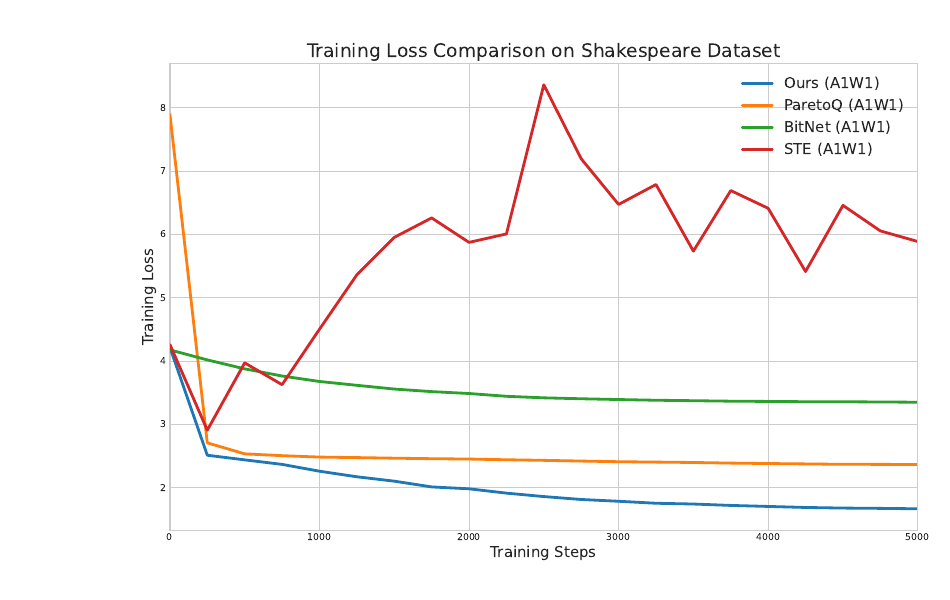
\includegraphics[width=\linewidth]{figs/fig1a_ste_divergence.png}\\[4pt]
\small Training loss, 1-bit weights and activations (A1W1), small GPT on Shakespeare. STE (red) diverges; the paper's method (blue) converges.
\end{minipage}\hfill
\begin{minipage}[t]{0.49\textwidth}\centering
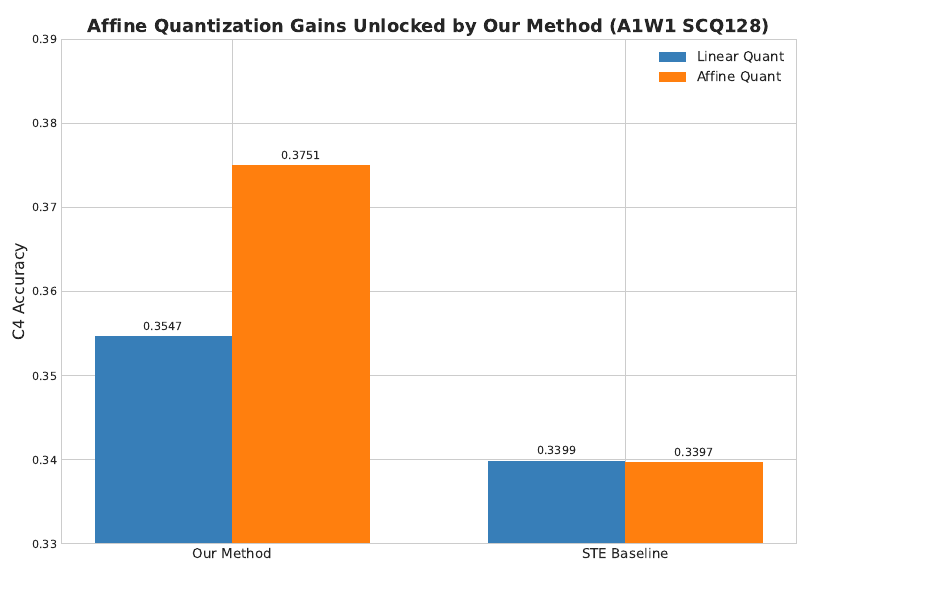
\includegraphics[width=\linewidth]{figs/fig1b_affine.png}\\[4pt]
\small Accuracy at A1W1, linear vs.\ affine quantization. Under STE affine gives no gain; with the paper's method it does.
\end{minipage}

\vfill
\noindent{\small\textit{Source:} Ye et al., ``Robust Training of Neural Networks at Arbitrary Precision and Sparsity,'' ICLR 2026, Fig.~1.}

\slide{The new approach: a denoising reconstruction $g$}

{\setlength{\abovedisplayskip}{3pt}\setlength{\belowdisplayskip}{3pt}
\paragraph{The change.} Keep $f$ and round. Replace $\hat x$ by a fitted reconstruction $g$.
\begin{itemize}\setlength{\itemsep}{3pt}
\item \textbf{Reconstruction.} A new affine map, fitted to $x$:
\[
\hat x=s_f\,q+b_f\mathbf 1\quad\longrightarrow\quad g(q)=s_g\,q+b_g\mathbf 1
\]
\item \textbf{Ridge regression objective.} Estimate $s_g$ and $b_g$ from the data:
\[
\min_{s_g,\,b_g}\ \frac{1}{2N}\big\|s_g\,q+b_g\mathbf 1-x\big\|^2+\frac{\lambda}{2}\,s_g^2
\]
\item \textbf{Solution.} Ridge regression has a closed form:
\[
s_g=\frac{\Cov_{xq}}{\Var_q+\hl{\lambda}},\qquad b_g=\bar x-s_g\,\bar q,\qquad \lambda=0.01
\]
{\centering\itshape \hl{\lambda} is the denoising knob.\par}
\end{itemize}

\paragraph{Forward pass.} The next layer gets $g(q)$, not $\hat x$.
\[
x\ \xrightarrow{\ f\ }\ f(x)\ \xrightarrow{\ \operatorname{round}\ }\ q\ \xrightarrow{\ g\ }\ g(q)\ \longrightarrow\ \text{rest of network}\ \longrightarrow\ L
\]

\paragraph{Backward pass.} Round stays straight through, as in STE. But $g$ now depends on $\delta$.
\[
\nabla_xL\ \xleftarrow[\text{straight through}]{\ \times\,1/s_f\ }\ \nabla_qL\ \xleftarrow[\text{depends on }\delta]{\ \times\,(\partial g/\partial q)^{\top}\ }\ \nabla_gL\ \longleftarrow\ \text{rest of network}\ \longleftarrow\ L
\]
}

\slide{Why it works: the Jacobian trick}

{\setlength{\abovedisplayskip}{6pt}\setlength{\belowdisplayskip}{6pt}
\paragraph{The idea.} Both methods guess round's gradient the same way. Only the Jacobian differs$^*$:
\[
J_{\text{STE}}=\frac{\partial}{\partial x}\big[s_f\,q+b_f\mathbf 1\big]=\underbrace{0}_{\text{exact}}+\underbrace{I}_{\text{guess}}
\qquad\qquad
J_{g}=\frac{\partial}{\partial x}\big[s_g(x,q)\,q+b_g(x,q)\,\mathbf 1\big]=\underbrace{P}_{\text{exact}}+\underbrace{\rho\,(I-P)}_{\text{guess}}+\underbrace{c\,u\,r^{\top}}_{\text{error}}
\]

\paragraph{The three parts of $J_g$.}
\begin{itemize}\setlength{\itemsep}{6pt}
\item \textbf{Exact.} Moving $x$ moves the fitted levels (the reconstruction levels):
\[
P=\frac{\mathbf 1\mathbf 1^{\top}}{N}+\frac{u\,u^{\top}}{N(\Var_q+\lambda)},\qquad u=q-\bar q\mathbf 1
\]
\item \textbf{Guess.} Scaled by $\rho$: the fitted scale $s_g$ over the grid scale $s_f$.
\[
\rho=\frac{s_g}{s_f}=0.29,\ \ 0.87,\ \ 0.99\qquad\text{at 1, 2, 4 bits}
\]
{\centering\itshape Coarse rounding gives a small $\rho$, so the guess counts less.\par}
\item \textbf{Error.} Carries the rounding error into the gradient:
\[
r=x-g(q),\qquad c=\frac{1}{s_fN(\Var_q+\lambda)}
\]
\end{itemize}
}

\vfill
\noindent{\small $^*$Derived by us, not in the paper. Checked against autograd. $\rho$ measured on a random block of 64 values.}

\slide{Results from the paper}

{\setlength{\abovedisplayskip}{3pt}\setlength{\belowdisplayskip}{3pt}
\paragraph{Small GPT on Shakespeare, 1-bit weights and activations.} STE's loss blows up; $g$ trains smoothly (slide 5).

\vspace{6pt}
\paragraph{Gemma 3 language model (1B), trained from scratch.} Score: share of next tokens predicted correctly.
\begin{center}
\renewcommand{\arraystretch}{1.3}
\begin{tabular}{lccc}
\toprule
bits for weights and activations & STE & with $g$ & gain \\
\midrule
4 & 0.425 & 0.427 & $+0.002$ \\
2 & 0.379 & 0.403 & $+0.023$ \\
1 & 0.340 & 0.375 & $+0.035$ \\
\bottomrule
\end{tabular}\par\vspace{8pt}
\textit{The fewer the bits, the bigger the gain.}
\end{center}
\begin{itemize}
\item \textbf{STE can diverge.} At 1.5 bits ($-1,0,1$), one STE run ends in NaN. $g$ still trains, reaching 0.330.
\end{itemize}

\vspace{16pt}
\noindent
\begin{minipage}[t]{0.48\textwidth}
\paragraph{Bigger model, fewer bits.} Quantized Gemma 3 4B beats 1B.\par\vspace{6pt}
\begin{itemize}\setlength{\itemsep}{6pt}
\item 4B, 1-bit weights, half pruned: 650 MB, score 0.452.
\item 1B, full precision: 1400 MB, score 0.449.
\end{itemize}
\end{minipage}\hfill
\begin{minipage}[t]{0.48\textwidth}
\paragraph{Other tasks, 4 bits, no extra tuning.} Matches full precision.\par\vspace{6pt}
\begin{itemize}\setlength{\itemsep}{6pt}
\item Images (ResNet-50): 76.45\% vs.\ 76.41\%.
\item Translation (English--German): 29.71 vs.\ 29.49 BLEU.
\end{itemize}
\end{minipage}
}

\slide{Toy implementation}

\noindent\textbf{Setup.} Character-level GPT (4 blocks, 0.82M parameters) on Tiny Shakespeare. All linear layers in the blocks quantized to $k$ bits (weights and activations, affine, per row); embeddings and output layer full precision. 3000 steps, same seed; only the dequantization differs: STE ($\hat x$) vs.\ ridge ($g$, $\lambda=0.01$), $k=1,2,4$.

\vspace{4pt}\noindent
\begin{minipage}[t]{0.49\textwidth}\centering
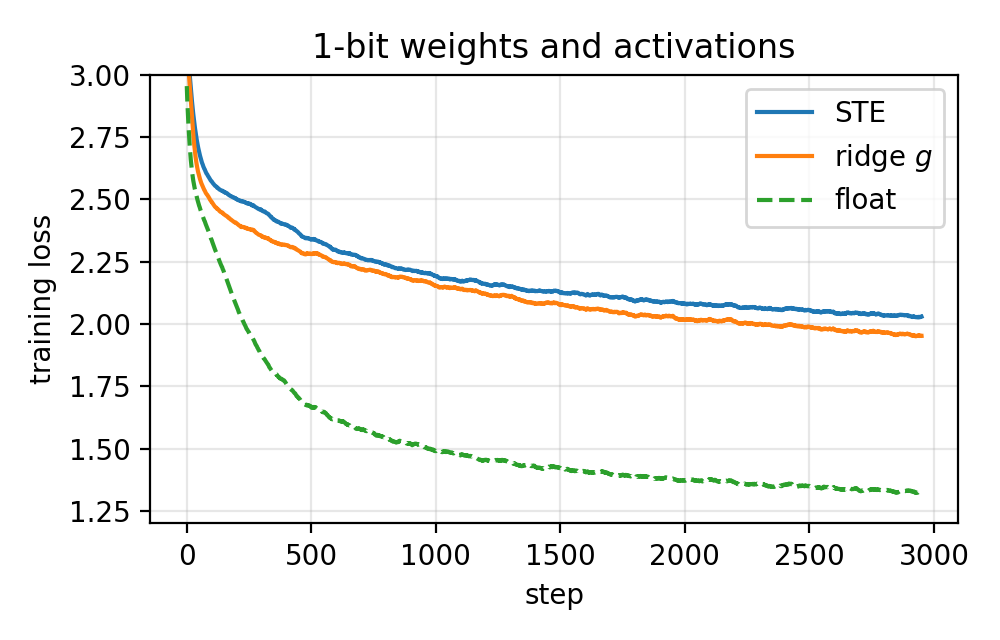
\includegraphics[width=0.9\linewidth]{implementation/plots/loss_k1.png}\\[2pt]
\small Training loss at A1W1.
\end{minipage}\hfill
\begin{minipage}[t]{0.49\textwidth}\centering
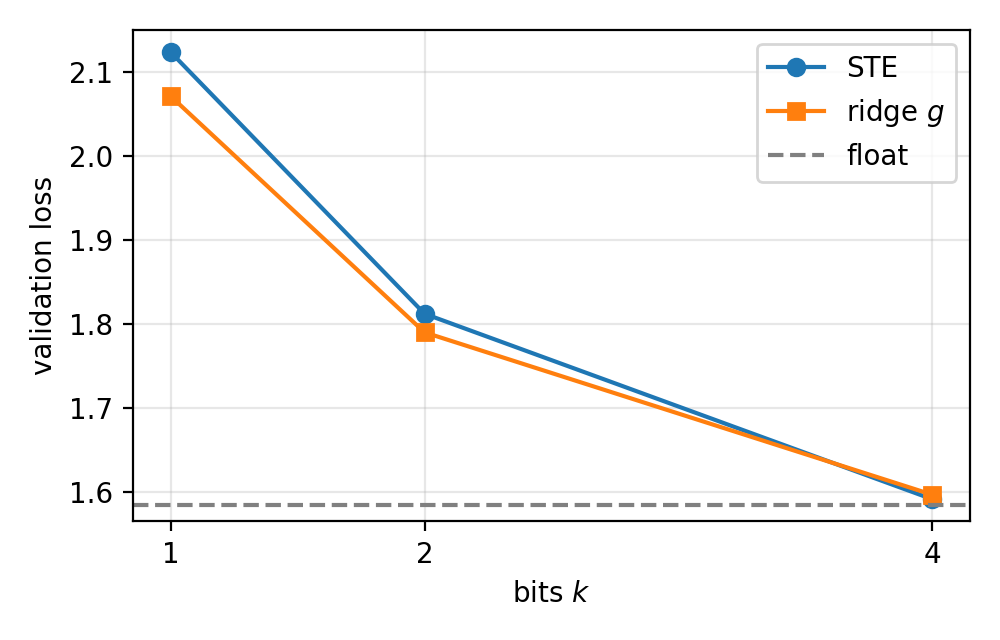
\includegraphics[width=0.9\linewidth]{implementation/plots/val_vs_bits.png}\\[2pt]
\small Final validation loss.
\end{minipage}

\vspace{6pt}\noindent
\textbf{Gradient check} (1 bit). Same $q$, $\delta$ changed by 0.106: the gradient reaching $x$ changes by 0.0000 under STE and 0.0144 under ridge.\\
\textbf{Size.} Float32 model 3.19 MB; at 1 bit 250 KB (12.7$\times$ smaller).

\vfill
\noindent{\small\textit{Reference:} model follows nanoGPT by A.~Karpathy, \texttt{github.com/karpathy/nanoGPT}.}

\slide{Advantages and disadvantages}

\vspace{14pt}
\noindent
\begin{minipage}[t]{0.48\textwidth}
\textbf{Advantages.}\par\vspace{-4pt}
\begin{itemize}\setlength{\itemsep}{20pt}
\point{Makes 1-bit training work.}{1-bit matmul is just XNOR + bit-count,\\[3pt]
\textit{$256\times$ cheaper than 16-bit.}\\[10pt]
STE can diverge there; $g$ trains smoothly.}
\point{Better reconstruction.}{Closer to $x$ than standard dequantization.}
\point{Extends to sparsity.}{Sparsity is quantization with small values thresholded to 0:\\[4pt]
$x\ \xrightarrow{\ \operatorname{threshold}\ }\ x_S\ \xrightarrow{\ f,\ \operatorname{round}\ }\ q\ \xrightarrow{\ g\ }\ g(q)$}
\end{itemize}
\end{minipage}\hfill
\begin{minipage}[t]{0.48\textwidth}
\textbf{Disadvantages.}\par\vspace{-4pt}
\begin{itemize}\setlength{\itemsep}{20pt}
\point{Round is still a guess.}{``Without gradient estimation'' is too strong.}
\point{Small gain at 4 bits.}{Only $+0.002$, \textit{in the most common setting.}}
\point{Extra storage.}{A scale and shift per 128 weights.}
\point{Savings are estimates.}{No real hardware, no speed numbers.}
\end{itemize}
\end{minipage}

\slide{Our takeaways}

\vspace{10pt}
\noindent
\begin{minipage}[t]{0.48\textwidth}
\textbf{What convinced us.}\par\vspace{14pt}
\plainpoint{A clean comparison.}{Only the reconstruction differs between the two methods.}
\plainpoint{Consistent gains.}{$g$ wins in every setting, more at fewer bits.}
\plainpoint{Our toy agrees.}{Better at 1--2 bits, a tie at 4 bits.}
\end{minipage}\hfill
\begin{minipage}[t]{0.48\textwidth}
\textbf{What we would question.}\par\vspace{14pt}
\plainpoint{``No gradient estimation''.}{The paper claims it (abstract; Table 8).\\[6pt]
But $\delta$ is detached, exactly as in STE:\\[9pt]
$q=f(x)+\operatorname{stopgrad}(\delta)\ \Rightarrow\ \partial q/\partial f(x)=I$}
\plainpoint{``For the first time''.}{LSQ (Esser et al., 2019) already puts $\delta$ in a gradient.}
\end{minipage}

\vspace{14pt}
\paragraph{What we would try next.} More seeds, a larger toy model, a sweep over $\lambda$.

\vfill
\noindent\fbox{\parbox{\dimexpr\textwidth-2\fboxsep-2\fboxrule}{\centering\large
\textbf{Takeaway:} Do not ignore the rounding error. Fit it.\\ A fitted reconstruction cleans the forward pass. It makes the backward pass error-aware.}}

\end{document}
